%%%
%% v3.3 [2020/05/14]
%\documentclass[Proof,technicalreport]{ieicej}
\documentclass[technicalreport]{ieicej}
\usepackage{graphicx}
%\usepackage[fleqn]{amsmath}
%\usepackage{amsthm}
%\usepackage{amssymb}
\usepackage{latexsym}
\usepackage{newtxtext}
\usepackage[varg]{newtxmath}
\usepackage{url}
\usepackage{amsmath}
\usepackage{autobreak}

\def\IEICEJcls{\texttt{ieicej.cls}}
\def\IEICEJver{3.2}
\newcommand{\AmSLaTeX}{%
 $\mathcal A$\lower.4ex\hbox{$\!\mathcal M\!$}$\mathcal S$-\LaTeX}
%\newcommand{\PS}{{\scshape Post\-Script}}
\def\BibTeX{{\rmfamily B\kern-.05em{\scshape i\kern-.025em b}\kern-.08em
 T\kern-.1667em\lower.7ex\hbox{E}\kern-.125em X}}

\jtitle{交差点における建物遮蔽とリンク状態を考慮した地理的opportunistic routing}
\etitle{Building Shadowing on Intersection and Link State aware Geographic Opportunistic Routing for Urban VANETs }
% \esubtitle{Guide to the Technical Report and Template}
\authorlist{%
 \authorentry[hanako@denshi.ac.jp]{高橋 柊人}{Shuto Takahashi}{BKC}% 
 \authorentry[taro@jouhou.co.jp]{吉田 政望}{Masami Yoshida}{BKC}% 
 \authorentry[jiro@jouhou.co.jp]{ガジェゴス ラモネト アルベルト}{Alberto Gallegos Ramonet}{gakubu}% 
 \authorentry[jiro@jouhou.co.jp]{野口 拓}{Taku Noguchi}{gakubu}%
}
\affiliate[BKC]{立命館大学情報理工学研究科\hskip1zw
  〒522-8577 滋賀県草津市野路東1-1-1}
 {Graduate School of Information Science and Engineering, Ritsumeikan University\hskip1em
  1-1-1 Noji-higashi, Kusatsu, Shiga 525-8577, Japan}
\affiliate[gakubu]{立命館大学情報理工学部\hskip1zw
  〒522-8577 滋賀県草津市野路東1-1-1}
 {College of Information Science and Engineering, 
  Ritsumeikan University\hskip1em
  1-1-1 Noji-higashi, Kusatsu, Shiga 525-8577, Japan}

% \MailAddress{$\dagger$is0361er@ed.ritsumei.ac.jp,
% $\dagger\dagger$\{taro,jiro\}@ritsumei.ac.jp}

\MailAddress{$\dagger$is0361er@ed.ritsumei.ac.jp,$\dagger$is0195hr@ed.ritsumei.ac.jp,$\dagger\dagger$ramonet@fc.ritsumei.ac.jp,$\dagger\dagger$noguchi@ed.ritsumei.ac.jp
}


\begin{document}
\begin{jabstract}
 複雑な都市環境での車両アドホックネットワーク(VANETs)では, 建物や樹木などの障害物が多数存在するため, シャドウイングやフェージングが起こり, 電波伝搬の妨害が発生する. しかし, 多くの既存opportunistic routingの性能評価では, シミュレーションでシャドウイングの影響が考慮されておらず, 通信性能が過大評価されている可能性がある. そこで, 本研究では, シャドウィングが既存 ルーチングプロトコル に与える影響をネットワークシミュレータ NS-3 のシャドウイングモデルであるObstacle Modelを用いて調査し, シャドウイングを考慮した新たな交差点ベースのルーチングプロトコル(SIGO) を提案する. SIGO は中継ノードの優先度を決定するため, 中継ノードと宛先ノードまでの距離, 中継ノードとの予想伝送確率に加えて, 交差点ノードであるかどうかを考慮する. シミュレーションにより, パケット到達率の向上と, エンドツーエンド遅延の減少を確認し, SIGO の通信性能の有効性を示した.
\end{jabstract}
\begin{jkeyword}
VANET,opportunistic routing, シャドウイング
\end{jkeyword}
\begin{eabstract}
In VANETs (Vehicle Ad Hoc Networks), the presence of many obstacles such as buildings and trees (complex urban environments) can interfere with the propagation of radio waves caused by shadowing and fading. However, most of the existing opportunistic routing systems do not consider shadowing into account in their simulations, which may lead to an overestimation of VANETs performance. In this study, we investigate the impact of shadowing on existing routing protocols using an obstacle model that implements the shadowing effect in the NS-3 network simulator. We propose a new intersection-based routing protocol (SIGO) that takes shadowing into account. To determine the priority of a relay node, SIGO protocol considers the distance between the relay node and the destination node, the probability of transmission to the relay node, and whether it is a node or not. The simulation results show that the communication performance of our SIGO protocol is effective in improving the packet delivery rate and reducing the end-to-end delay.
\end{eabstract}
\begin{ekeyword}
VANET, opportunistic routing, shadowing
\end{ekeyword}
\maketitle

\section{まえがき}


自動車運転の安全性や利便性の向上, 環境負担の低減を目的とし, 高度交通システム(Intelligent Transportations System : ITS) \cite{ITS} に関する取り組みが盛んにおこなわれている. 車車間通信を利用して形成される車両アドホックネットワーク(Vehicle Ad Hoc Networks: VANETs) は, ITSにおける多様なアプリケーションの実現に必要不可欠である. VANETsでは, 無線通信機を搭載した車車間でアドホック通信を行うことで, リアルタイム性と柔軟性を持つネットワーク構築が可能となる. しかし,  ITSシステムを安定してサポートするためには, 通信オーバーヘッドの削減, 高いパケット到達率, リアルタイム性を実現するルーチングプロトコルが必要となる. \par
 都市環境での車両ネットワークでは, ノードのモビリティや建物の存在を考慮する必要があり, 典型的なrouting手法\cite{Old1},\cite{Old2}では, ノードの高速なモビリティへの対応が課題とされている[4]. これらの手法に対して, opportunistic routingが注目を集めている\cite{EXOR}. opportunistic routingと従来のroutingの最大の違いは, 固定ルートを使用せず, パケットを受信したノードが再転送するか否かを自己選択する点である. これにより, 従来のrouting方式に比べて, opportunistic routingは中継パケットを受信する機会を増やし, 結果として優れたパフォーマンスを実現できることを示している.\par
 しかし, 既存のopportunistic routingの多くは,都市環境を想定して考案されているが, 性能評価で建物によるシャドウイングの影響が考慮されておらず,通信性能を過大評価している可能性がある.
 
 そこで本研究では, 既存opportunistic routingであるLSGO\cite{LSGO}をネットワークシミュレータNS-3のシャドウイングモデルであるObstacle Model\cite{Obstacle}を用いて評価し, 建物によるシャドウイングが起こる場合と起こらない場合の通信性能を検証する. また, シャドウイングが起こる環境での通信性能の向上を目的とした新たなルーチングプロトコル(SIGO)を提案する. SIGOは中継ノード選択する際に, 宛先ノードまでの距離, 伝送確率に加えて, 交差点のノードであるかどうかを考慮する. 提案手法の有効性をシャドウイングが考慮されたシミュレーション環境で評価する.\par
 2章では既存opportunistic routingを紹介し課題点を述べ, 3章では提案手法について紹介し, 4章ではシミュレーションでLSGO protocolのシャドウイングが起こる場合の通信性能への影響の評価と, 提案手法の有効性について示す. 最後に5章でまとめと今後の課題について述べる.


\section{関連研究}

近年, opportunistic routingが注目を集めている. これは従来のgeographic routing \cite{GPSR}\cite{GPCR}などに比べ, 中継ノードがパケット受信する機会を増やすことで通信性能の向上を果たしている. opportunistic routingの基本モデルを図\ref{fig:Basic}に示す.ノード$N_{s}$が送信ノード, $N_{d}$が宛先ノードである. 送信ノード$N_{s}$は中継候補ノードとして, $N_{1}$ ~ $N_{n}$を選択し, 選択したノードそれぞれに優先順位を指定してパケットを送信する. 受信した$N_{1}$ ~ $N_{n}$のノードはそれぞれ自身の優先順位を確認し, 優先順位の高いノードから再転送を行う. また, 各中継ノードは自身より優先度の高いノードの再転送を受信すると自身の再転送をキャンセルし, 冗長なパケットの増加を防いでいる. これらのことから, opportunistic routingにおいて, 優先度決定アルゴリズムが通信性能に直接影響を及ぼすことがわかる.\par
代表的なopportunistic routing としてEXOR\cite{EXOR}が提案されている. これは, 中継ノードの優先度を, ETX\cite{ETX}と類似した独自の予想伝送コストを用いて決定している. しかし, この新たに考案されたETX値は, VANETの性質であるノードのランダムで高速なモビリティを考慮していないという問題がある.\par
そこで, 新たにVANETに適したETX値を考案したLSGO\cite{LSGO}が提案された. LSGOでは, 予想伝送コストと呼ばれるVANET用に最適化されたETX値を, 優先度を決定する指標として使用し, パケット到達率の向上, エンドツーエンド遅延の減少を実現しいる. また, SCAOR\cite{SCAOR}では, パケットの衝突でネットワークのパフォーマンスを低下させる問題を防ぐために, ノード密度パラメータを, 優先度決定における指標として追加し, LSGOやEXORに比べ通信性能が向上することを示している.\par
 しかし, これらのprotocol に共通する課題として, シミュレーションの性能評価として, 建物によるシャドウイングが考慮されていないことが挙げられる. この問題によりこれらのprotocol は通信性能を過大評価している可能性がある. 本研究では, LSGOについて, シミュレーションを用いて, シャドウイングを考慮した場合の通信性能への影響を検証する. 
 \begin{figure}[!ht]
\centering
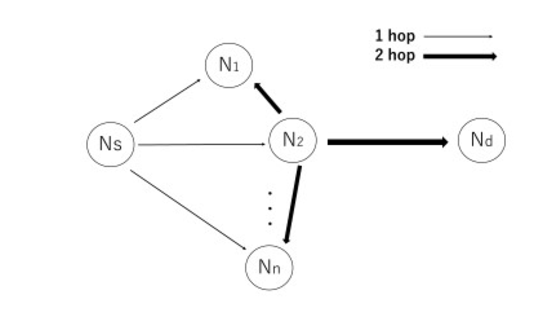
\includegraphics[width=90mm]{figures/basic-opportunity.eps}
\caption{opportunistic routingの基本モデル}
\label{fig:Basic}
\end{figure}



\section{提案手法}
本研究では, 中継ノードを選択し, 優先度を決定するための指標として, 宛先ノードまでの進度( 送信ノードに比べてどれだけ宛先ノードに近いか), リンク状態, 交差点度数の3つの指標を用いたSIGOを提案する. 

\subsection{概要}
SIGOでは, 各ノードは定期的に自ノードのID, X座標, Y座標で構成されたHelloパケットをブロードキャストする. 送信ノードは宛先ノードにパケットを届けるために, Helloパケットの情報をもとに, 近隣ノードの中から中継候補ノードを複数選択し, それらに優先度をつけて以下の中継パケットをブロードキャストする. 中継パケットのフォーマットを図\ref{fig:Packet} に示す.
% \begin{table}[!ht]
% \begin{center}
% \caption{中継パケットフォーマット}
% \label{tab:packet}
% \begin{tabular}{|l|l|l|l|l|l|l|l|l|}
% \cline{1-9}
% $DesID$ & $Xpos$ & $Ypos$ & $ID_{1}$ & $ID_{2}$ & $ID_{i}$ & .... &  $ID_{N}$ & $Data$ \\ \cline{1-9}
% \end{tabular}
% \end{center}
% \end{table}

\begin{figure}[!ht]
\centering
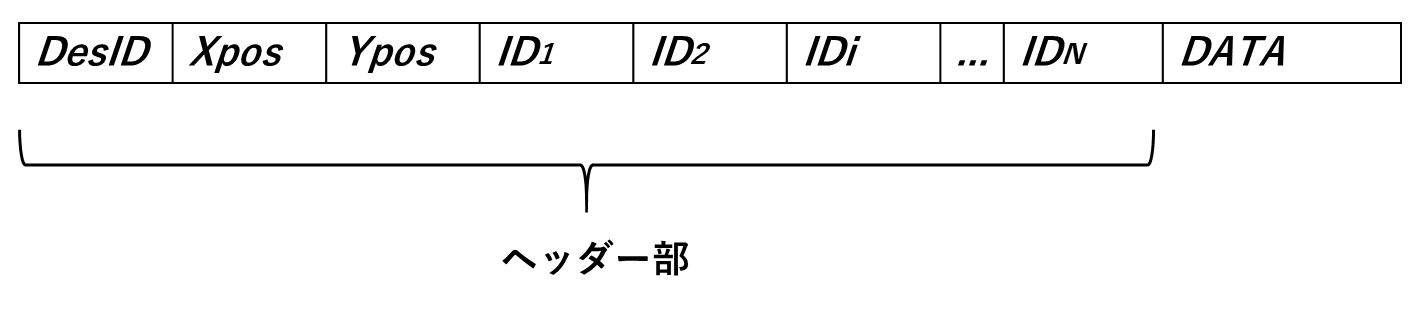
\includegraphics[width=90mm]{figures/Packet.eps}
\caption{中継パケットのフォーマット}
\label{fig:Packet}
\end{figure}

$DesID$は宛先ノードのID, $Xpos$, $Ypos$ は宛先ノードの位置情報, $DATA$は中継パケットのペイロード部を表している. 宛先ノードの位置情報の取得方法は, 何らかの位置情報サービスを利用するものとし本研究では検討対象外とする. $ID_{1}$  ~ $ID_{N}$は中継候補ノードのIDを表している. 候補ノードの個数や優先順位は, 後述するアルゴリズムに従い送信ノードが決定する. 中継パケットを受信した各ノードは, 自ノードのIDが含まれているかを確認し, 含まれない場合はパケットを破棄する. 含まれている場合は, 自ノードの優先順位を確認し, 3.4節で述べるアルゴリズムに従い, 再転送を行うか否かを決定する. 



\subsection{リンクの品質の推定}
SIGOでは, 各ノードがHelloパケットを定期的にブロードキャストし, それを用いてリンク状態ETXを推定する. Helloパケットは, 自ノードのID, X座標, Y座標で構成されている. ETXを算出するために, 各ノードは近隣ノードから最初にHelloパケットを受信した時間$t_{0}$を記録する. そして, 現在時刻を$t$, ウィンドウサイズを$w$(second), Helloパケットの送信間隔を$τ$とすると, 予想伝送確率$r(t)$はウィンドウサイズ$w$で場合分けされ, 式(\ref{trans-prediction})で算出される.
\begin{equation}
\label{trans-prediction}
r(t) =\begin{cases}count(t, t_{0}), & 0 < t - t_{0} < 1,  \\ \frac{count(t,t_{0})}{(t-t_{0}) / τ}, & 1 \leq t - t_{0} \leq w\\
\frac{count(t - w,t)}{w / τ}, &  t - t_{0} \geq w\\
\end{cases}
\end{equation}



ウィンドウサイズ$w$は, $r(t)$を算出する際に, 現在時刻$t$より以前に取得したHelloパケットの有効期間である. 例えば, 現在時刻$t$=10(s), ウィンドウサイズ$w$=5(s)とすると, 時刻5(s)より古いHelloパケットの情報は$r(t)$を算出する際には用いない. $(t,t_{0})$ / $τ$は, ウィンドウサイズの間に受信されるべきHelloパケット数であり, $count(t,t_{0})$は$t$ ~ $t_{0}$の期間中に実際に受信されたHello パケットの数である. \par
 各近隣ノードとのリンクの非対称性は考慮せず, 一方向の予想伝送確率$r(t)$のみを使用してETXを計算する. 一方向伝送確率が$r(t)$であると仮定すると, リンクETXは式(\ref{equ-intersection})で算出される.
 
 \begin{equation}
 \label{equ-intersection}
 ETX = \frac{1}{  {r(t)}^{2}   } 
 \end{equation}

\subsection{交差点度数}
SIGOでは, 建物によるシャドウイングの影響を最小限にするため, 交差点ノードが優先的に中継ノードとして選択される指標を追加する. 交差点度数は以下の式(3)で算出される.

\begin{equation}
 交差点度数 = αθ
 \end{equation}
 
  $θ$は送信ノードと 宛先ノードを結ぶ直線と,送信ノードと交差点ノードを結ぶ直線のなす角である(図\ref{fig:Intersection}). 
  $θ$が大きくなるほど, 交差点度数は大きくなり, 次節で述べる優先度決定アルゴリズムにより交差点ノードが優先される可能性が増加する. $α$は, 交差点度数の重み付けであり, この値が増加するほど交差点度数が増加し, 交差点ノードが優先される確率が増加する. 
 
 \begin{figure}[!ht]
\centering
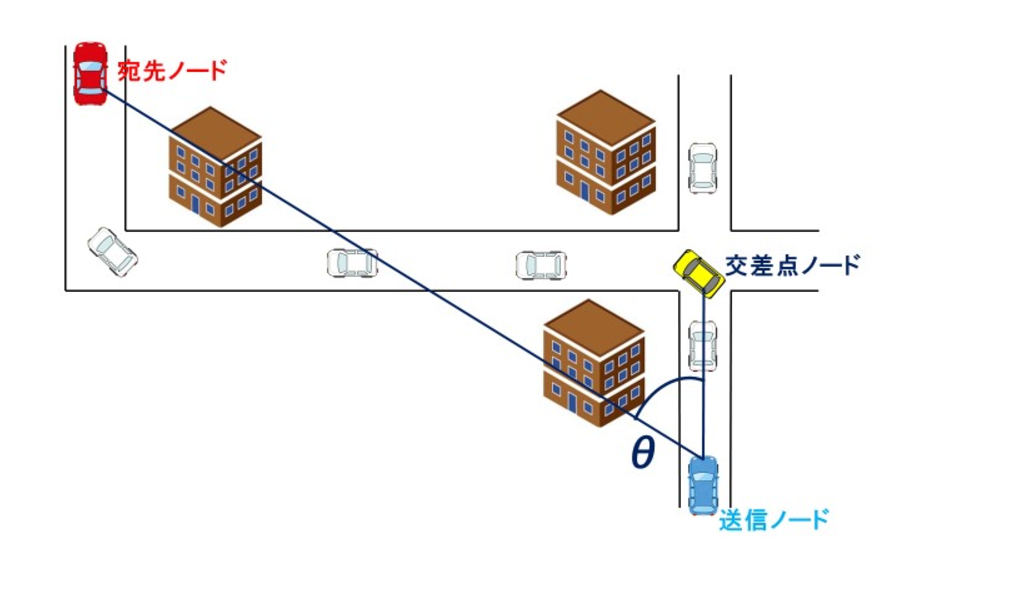
\includegraphics[width=90mm]{figures/Intersection.eps}
\caption{交差点度数}
\label{fig:Intersection}
\end{figure}

\subsection{優先度スケジューリングアルゴリズム}
SIGOでは, タイマーベースの優先度スケジューリングアルゴリズムを使用する. このアルゴリズムでは, 最も優先度が高いノードが最初にパケットを送信する. ほかの候補ノードは, 優先順位の高いノードからのパケットを受信すると, 自身のパケットを破棄する. タイマーが期限切れになり, 自身より優先度の高いノードからのパケットを受信していない場合, 送信を開始する. SIGOは以下の式(\ref{pri-intersection})(\ref{pri})によって, ノード$i$の優先度が算出される.


\begin{equation}
\label{pri-intersection}
\frac{D_{sd} - D{id}}{ETX_{i}^{2}} \times αθ,  D{id} < D_{sd}
\end{equation}

\begin{equation}
\label{pri}
\frac{D_{sd} - D{id}}{ETX_{i}^{2}} ,   D{id} < D_{sd}
\end{equation}

$D_{sd}$は送信ノードから宛先ノードまでの距離, $D_{id}$は候補ノード$i $から宛先ノードまでの距離である.  $D{id}$ < $D_{sd}$の条件を満たさない場合は, 優先度の計算を行わずに中継候補ノードから除外する. 式(\ref{pri-intersection})はノード$i$が交差点ノードの場合, 式(\ref{pri})は交差点ノード以外に位置する場合に適用される. 式(\ref{pri-intersection})または(\ref{pri})で算出された値が大きいほどノード$i$の優先順位が高くなる. 



\subsection{中継候補ノード選択アルゴリズム}
SIGOは, 信頼性を確保しながら, 送信回数を減らすために中継候補ノード数を最適化する必要がある. 式(\ref{pri-intersection})(\ref{pri})を用いて各隣接ノードの優先順位を$p$ = 1,2..N(1が最も優先順位が高い)とすると, $N$は次の条件を満たす必要があり, 候補ノードは1~$N$に制限される. 
\begin{equation}
\label{Min-Probability}
1 - \prod_{p=1}^N (1 - r_{p}(t))\geq R
\end{equation}

% \begin{eqnarray}
% \label{prifda}
% d_{1}(t)  \geq   d_{2}(t) \geq   d_{i}(t)   \geq d_{i}(t)    \geq  d_{N}(t) 
% \end{eqnarray}


式(\ref{Min-Probability})における$r_{p}(t)$ (1$ \leqq $p$ \leqq $N)は, 送信ノードが保持する隣接ノード(優先順位$p$)に対する予想伝送確率である. 
式(\ref{Min-Probability})の左辺は送信ノードからのパケットを候補ノード1~$N$のいずれかのノードが受信すると予想される確率であり, 右辺$R$はその確率の閾値である. $R$が大きいほど, 中継候補ノード数が増加し, 小さくなるほど, 候補ノード数が減少する. 車両密度が小さい場合や送信ノードと各隣接ノード間の予想伝送確率が低い場合, 式(\ref{Min-Probability})満たすことができない場合がある. その場合, $D{id}$ < $D_{sd}$の条件を満たすすべての隣接ノードが候補ノードとして選択される. また, 送信ノードと各隣接ノードとの予想伝送確率が高い場合, 候補ノード数$N$は小さくなるため, 信頼性を確保しながら, 最低限の候補ノード数を選択することができる. 





\section{性能評価}
性能評価では, ネットワークシミュレータNS-3[12]と交通流シミュレータSUMO[13] を用いて評価を行う. また, シャドウイングの影響をシミュレーションで考慮させるため, 電波減衰モデルとしてObstacle shadowing model [7]を用いた. 4.2節でシャドウイングによる電波減衰の有無による通信性能の違いを評価し, 4.3節でSIGOの性能評価を行う.


\subsection{シミュレーション設定}
シミュレーションパラメータを表\ref{tab:parameter}, シミュレーションシナリオを図\ref{fig:big-scenario}, 図\ref{fig:small-scenario}に示す. シミュレーション開始時に, ランダムな送信ノードと宛先ノードがそれぞれ20台ずつ割り当てられ, 通信を開始する. 
\begin{table}[!ht]
\begin{center}
\caption{シミュレーションパラメータ}
\label{tab:parameter}
\begin{tabular}{|l|l|lll}
\cline{1-2}
Simulation area    & 2100m × 2100m   &  &  &  \\ \cline{1-2}
Mobility model     & Random mobility &  &  &  \\ \cline{1-2}
Transmission range & 250m            &  &  &  \\ \cline{1-2}
Number of vehicles & 300 ~ 1000      &  &  &  \\ \cline{1-2}
Weight value ($α$) & 0.07      &  &  &  \\ \cline{1-2}
\end{tabular}
\end{center}
\end{table}

\begin{figure}[!ht]
\centering
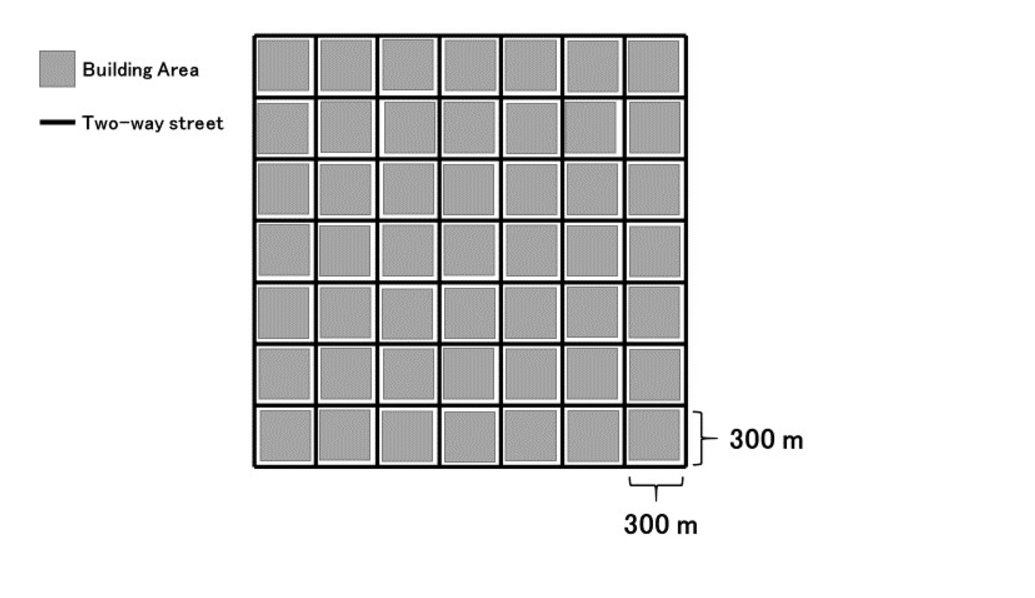
\includegraphics[width=90mm]{figures/big-scenario.eps}
\caption{建物が多いシミュレーションシナリオ}
\label{fig:big-scenario}
\end{figure}

\begin{figure}[!ht]
\centering
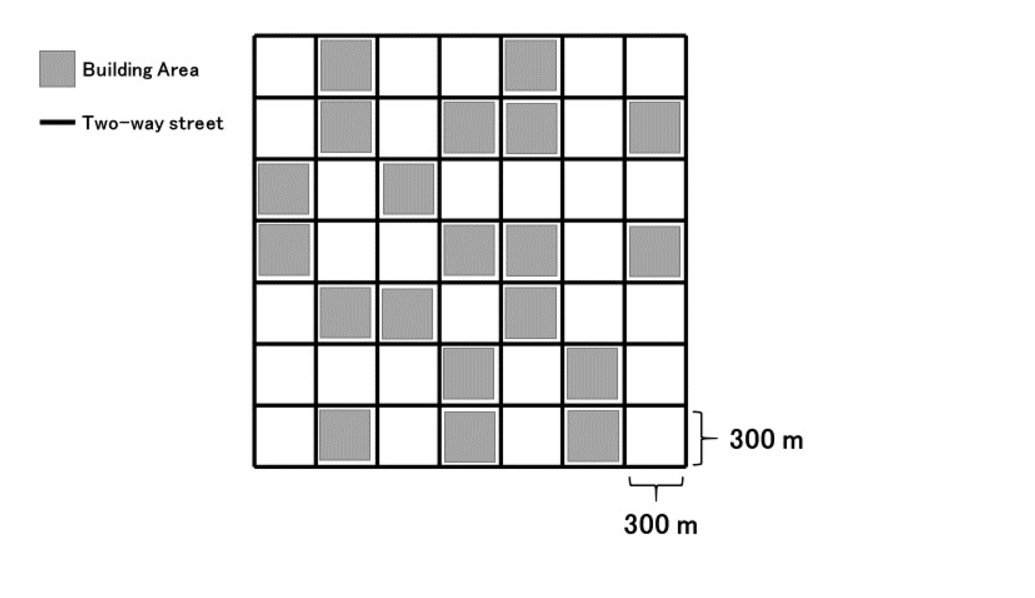
\includegraphics[width=90mm]{figures/small-scenario.eps}
\caption{建物が少ないシミュレーションシナリオ}
\label{fig:small-scenario}
\end{figure}

\par

\subsection{LSGOにおけるシャドウイングの影響}
シミュレーションで建物のシャドウイングによる電波の減衰が起こる場合のLSGOの通信性能に与える影響を, パケット到達率, エンドツーエンド遅延, オーバーヘッドの3つの評価項目で評価した. 
図\ref{fig:PDR-shadowing}はネットワークシミュレータでシャドウイングの影響を考慮した場合としない場合とでの, パケット到達率を示している. パケット到達率は, 送信ノードが送信した合計パケット数に対する, 宛先ノードが受信したパケット数の合計の比率である. 図\ref{fig:PDR-shadowing}では, シミュレーションでシャドウイングを考慮した場合, 全てのノード数においてパケット到達率が減少している. これは, シャドウイングによる電波減衰が原因だと推測される.

\begin{figure}[!ht]
\centering
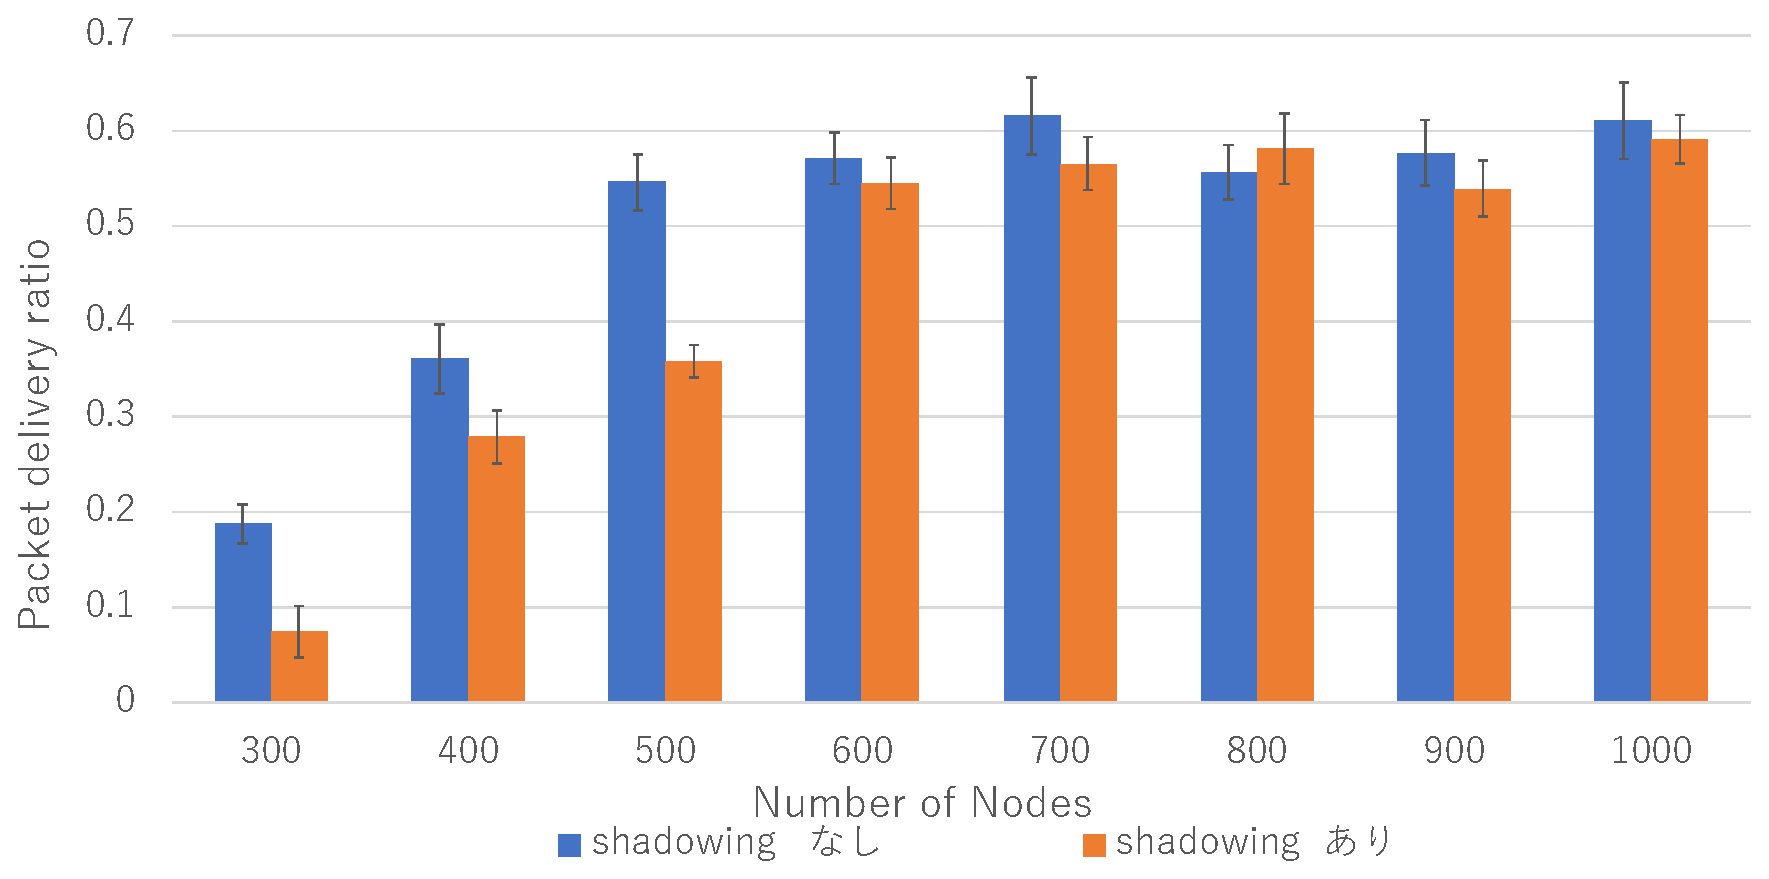
\includegraphics[width=90mm]{figures/PDR-shadowing.eps}
\caption{パケット到達率 シャドウイングの有無}
\label{fig:PDR-shadowing}
\end{figure}

図\ref{fig:Delay-shadowing}はネットワークシミュレータでシャドウイングの影響を考慮する場合としない場合とでのエンドツーエンド遅延(秒)を示している. エンドツーエンドの遅延は送信ノードがパケットを送信してから宛先ノードが正常に受信するまでにかかる平均時間として定義する. 図\ref{fig:Delay-shadowing}では, シミュレーションでシャドウイングを考慮した場合, 全てのノード数においてエンドツーエンド遅延が増加している. これはシャドウイングによる電波減衰が起こり, 建物を通過するパケットが届きにくくなることで, 送信ノードと宛先ノードを直線的に結ぶような経路が形成することが難しくなったことが原因だと考えられる. 

\begin{figure}[!ht]
\centering
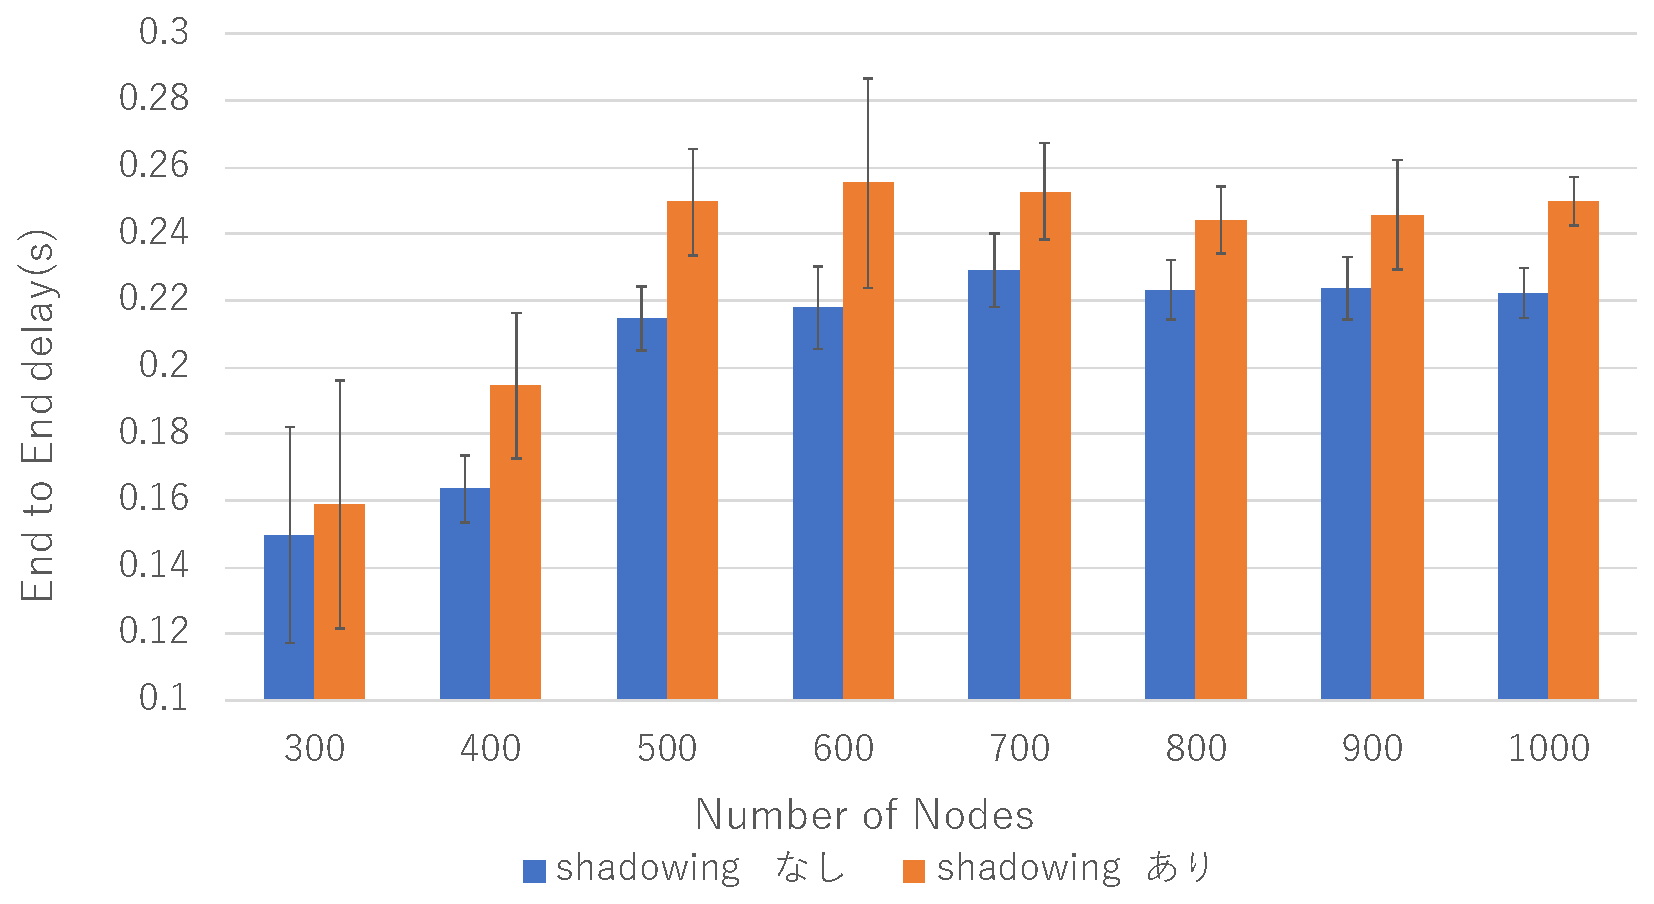
\includegraphics[width=90mm]{figures/Delay-shadowing.eps}
\caption{エンドツーエンド遅延 シャドウイングの有無}
\label{fig:Delay-shadowing}
\end{figure}


図\ref{fig:Overhead-shadowing}はネットワークシミュレータでシャドウイングの影響を考慮した場合としない場合とでの, オーバーヘッドを示している. オーバーヘッドはネットワーク全体における各ノードが送信したパケット数の合計を各ノードが正常に受信したパケット数の合計で割ったものである 図\ref{fig:Overhead-shadowing}では, シミュレーションでシャドウイングを考慮した場合, すべてのノード数においてオーバーヘッドが増加している. これは, opportunistic routing での送信ノードから指定された候補ノード同士が自分より優先度の高いノードからのパケットを建物による電波減衰によって, 受け取れない確率が増加し, 再転送がキャンセルされていないことが原因だと推測される. 


\begin{figure}[!ht]
\centering
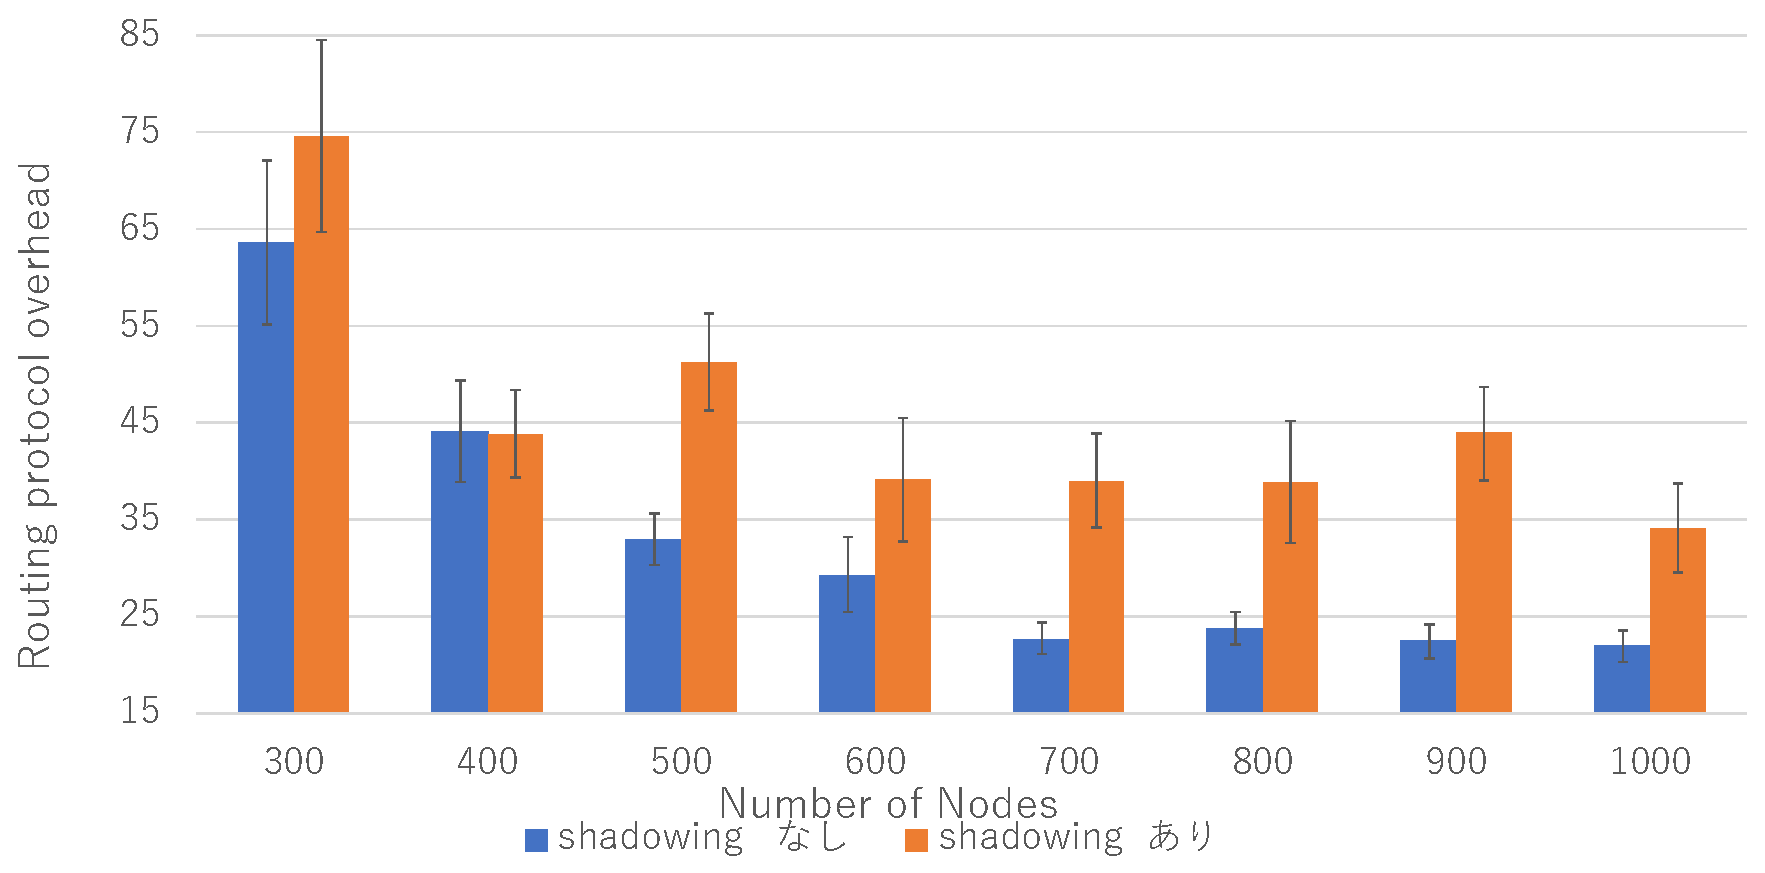
\includegraphics[width=90mm]{figures/Overhead-shadowing.eps}
\caption{オーバーヘッド シャドウイングの有無}
\label{fig:Overhead-shadowing}
\end{figure}


\subsection{SIGOの評価}
提案手法の有用性を評価するために, 4.2章と同様にパケット到達率, エンドツーエンド遅延, オーバーヘッドの3つの評価項目でLSGO protocolとの比較を行った. さらに, 図\ref{fig:big-scenario}, 図\ref{fig:small-scenario}のシミュレーションシナリオで評価し, 建物の多さによる評価を行った. 

図\ref{fig:PDR}は建物が多い場合と, 建物が少ない場合でのSIGOとLSGOのパケット到達率を示している. 図\ref{fig:PDR}では, 建物が多いシナリオでは, SIGOはLSGOに比べてパケット到達率の向上していることがわかる. これはSIGOでは, 交差点ノードの優先度が高くなる可能性が高まり, よりシャドウイングの影響を受けにくいルートが形成することができているからだと推測される. 
一方, 建物が少ないシナリオではSIGOはLSGOに比べてパケット到達率の安定した向上は得られなかった. これは, シャドウイングの影響が少ないシナリオでは, 交差点ノードを優先させる利点が少なかったことが原因として推測される. 

\begin{figure}[!ht]
\centering
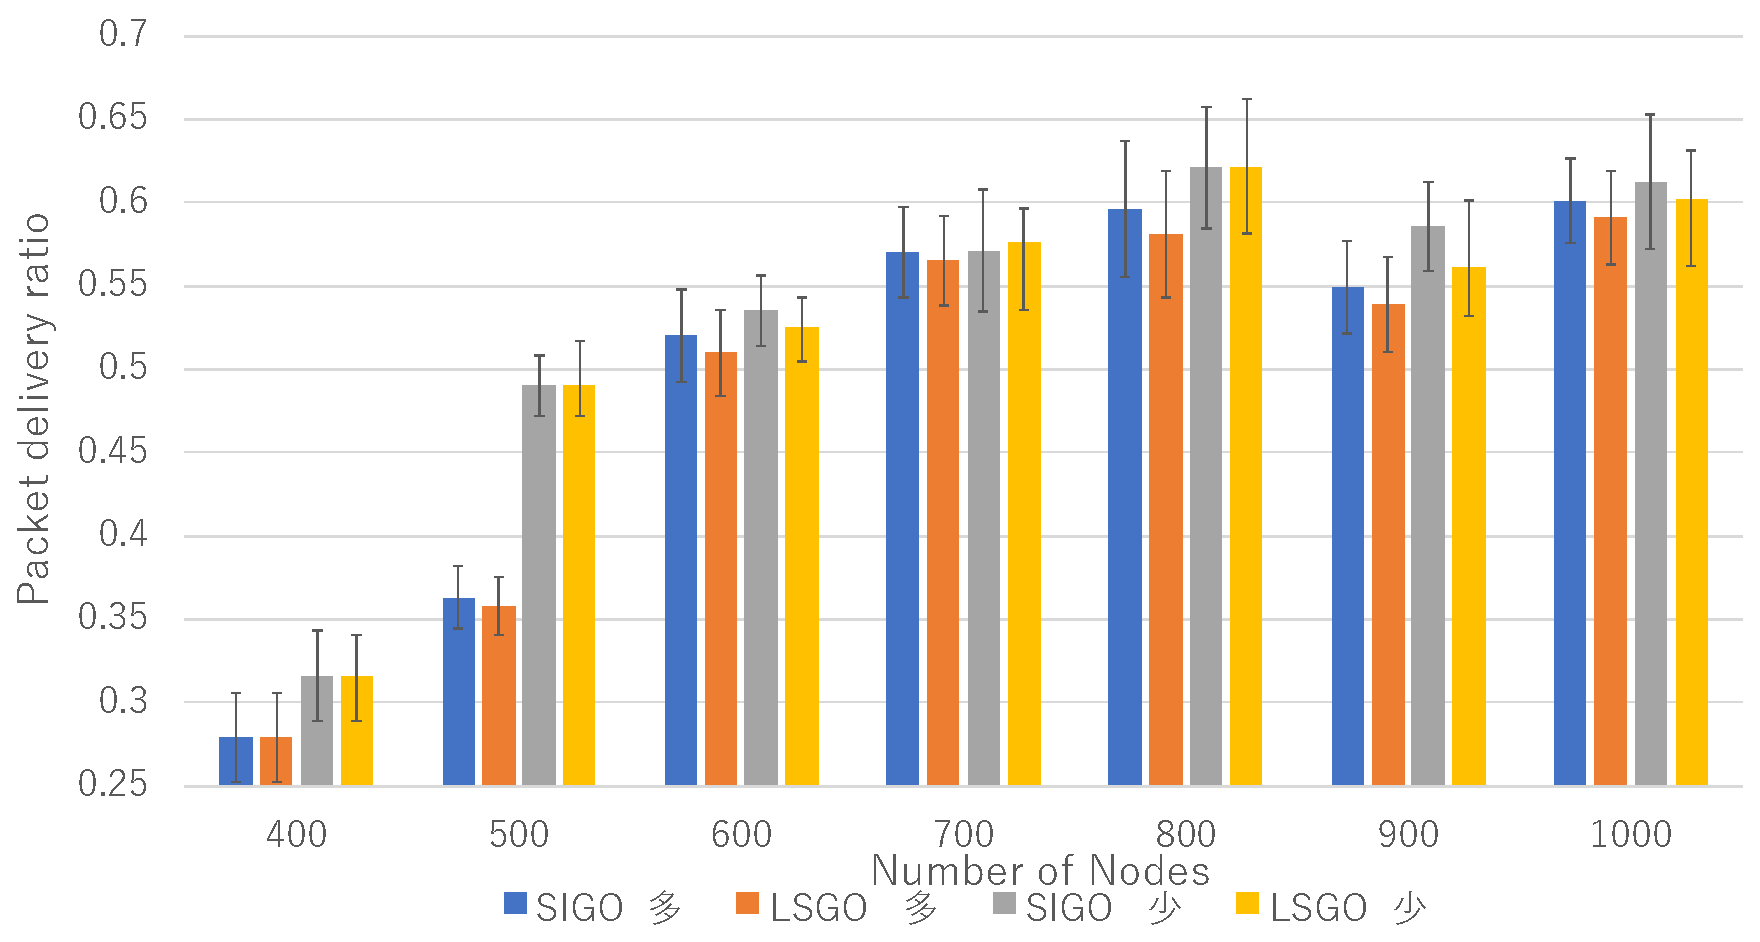
\includegraphics[width=90mm]{figures/PDR.eps}
\caption{パケット到達率 LSGO vs SIGO}
\label{fig:PDR}
\end{figure}


 図\ref{fig:Delay}は建物が多い場合と, 建物が少ない場合でのSIGOとLSGOエンドツーエンド遅延を示している. 建物が多い場合は, SIGOはLSGOに比べてエンドツーエンドの遅延が減少していることがわかる. これは, 交差点ノードの優先度が高くなる可能性が高まり, よりシャドウイングの影響を受けにくく, 候補ノードへパケットが正常に伝搬される可能性が高まることで, 優先度が高く, 待ち時間が短いノードがパケットを中継している確率が高いことが原因だと推測される. 一方, シャドウイングの影響が少ないシナリオでは, LSGOに比べて遅延が増加していることがわかる. これは交差点ノードがシャドウイングの影響が少ないにもかかわらず優先され, ホップ数が増加していることが原因として推測される. 
 
 \begin{figure}[!ht]
\centering
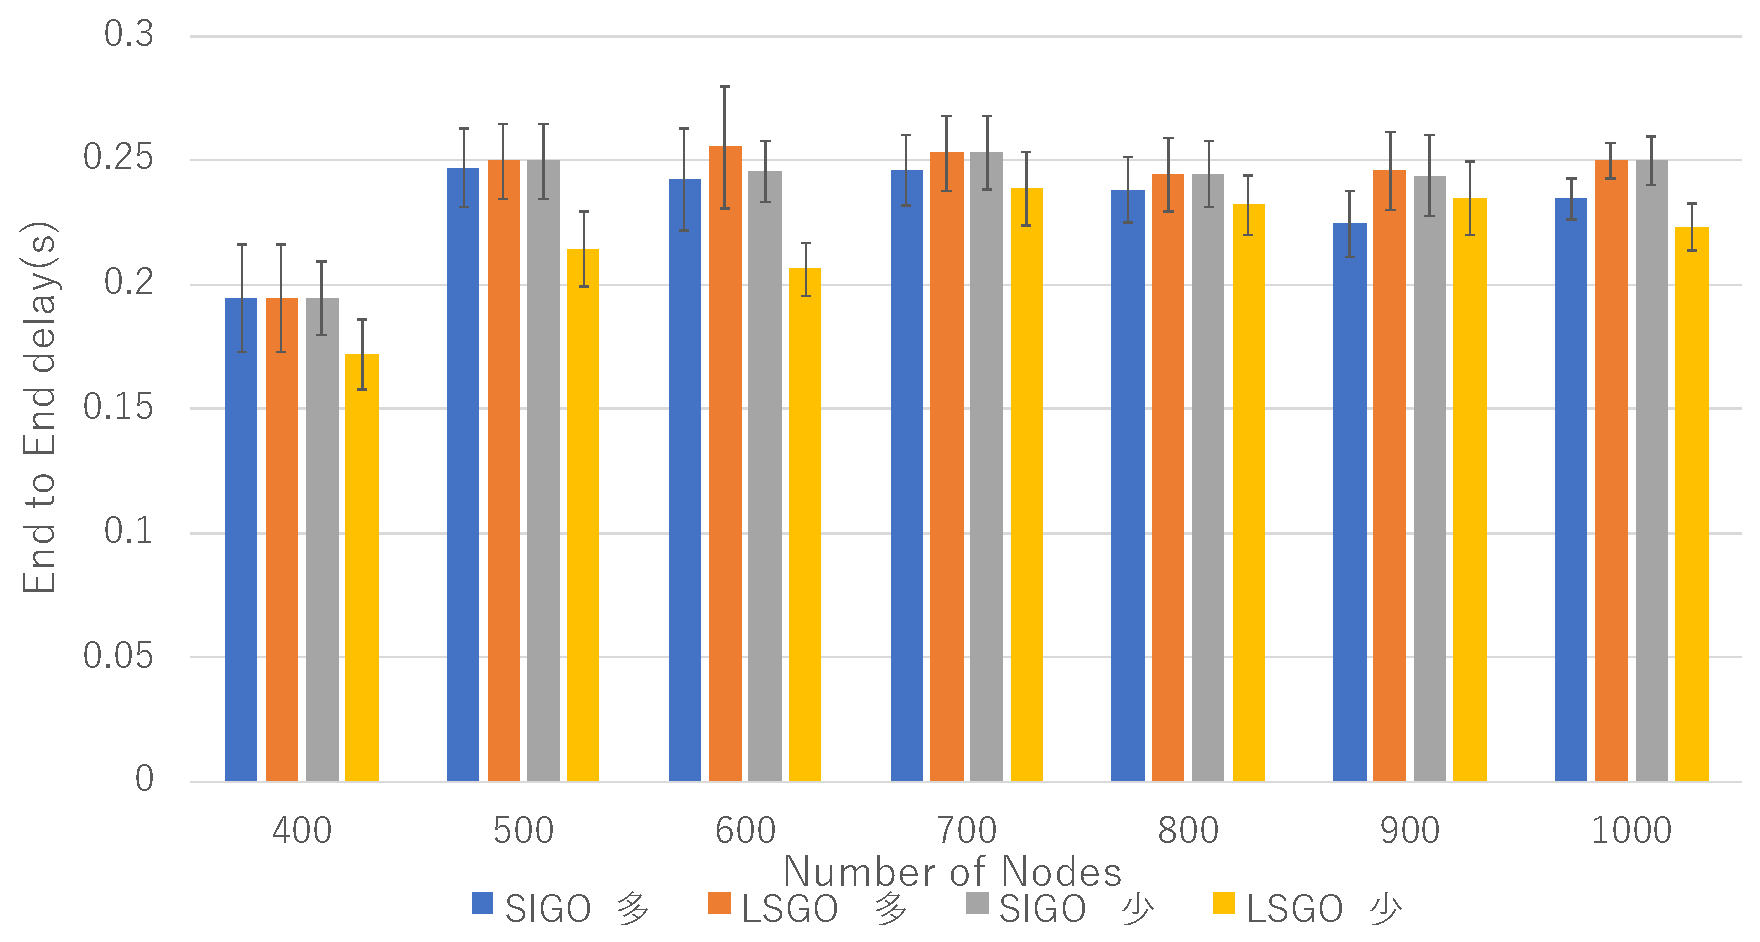
\includegraphics[width=90mm]{figures/Delay.eps}
\caption{エンドツーエンド遅延 LSGO vs SIGO}
\label{fig:Delay}
\end{figure}

図\ref{fig:Overhead}は建物が多い場合と, 建物が少ない場合でのSIGOとLSGOのオーバーヘッドを示している. SIGOはLSGOに比べて建物が多いときと少ないとき, どちらの場合もオーバーヘッドが増加してしまっていることがわかる. これはLSGOに比べてSIGOでは交差点ノードが優先される確率が高く, 比較的道に沿ってパケットが中継されるため, ホップ数が増加したと推測される. また, 宛先ノードの方向に建物が存在し, 交差点ノードがパケットを中継した場合, 交差点を形成する2つの異なる道路に存在するノードが候補ノードとして選択される.この状況では,優先順位の低い候補ノードが優先順位の高い候補ノードからのパケットをシャドウイングの影響で受け取れない可能性が増加し,再転送がキャンセルされずに冗長なパケット転送が増加してしまう. 図\ref{fig:Overhead-reason}に例を示す.交差点ノードが中継したパケットはノード1-4が受信し, 候補ノードの優先順位はノード1から順に設定される.本来はノード1のみが中継を行うことが理想であるが, ノード1がパケットを送信しても, ノード3, 4はシャドウイングの影響で受信することができず, 再転送を行ってしまう.

 \begin{figure}[!ht]
\centering
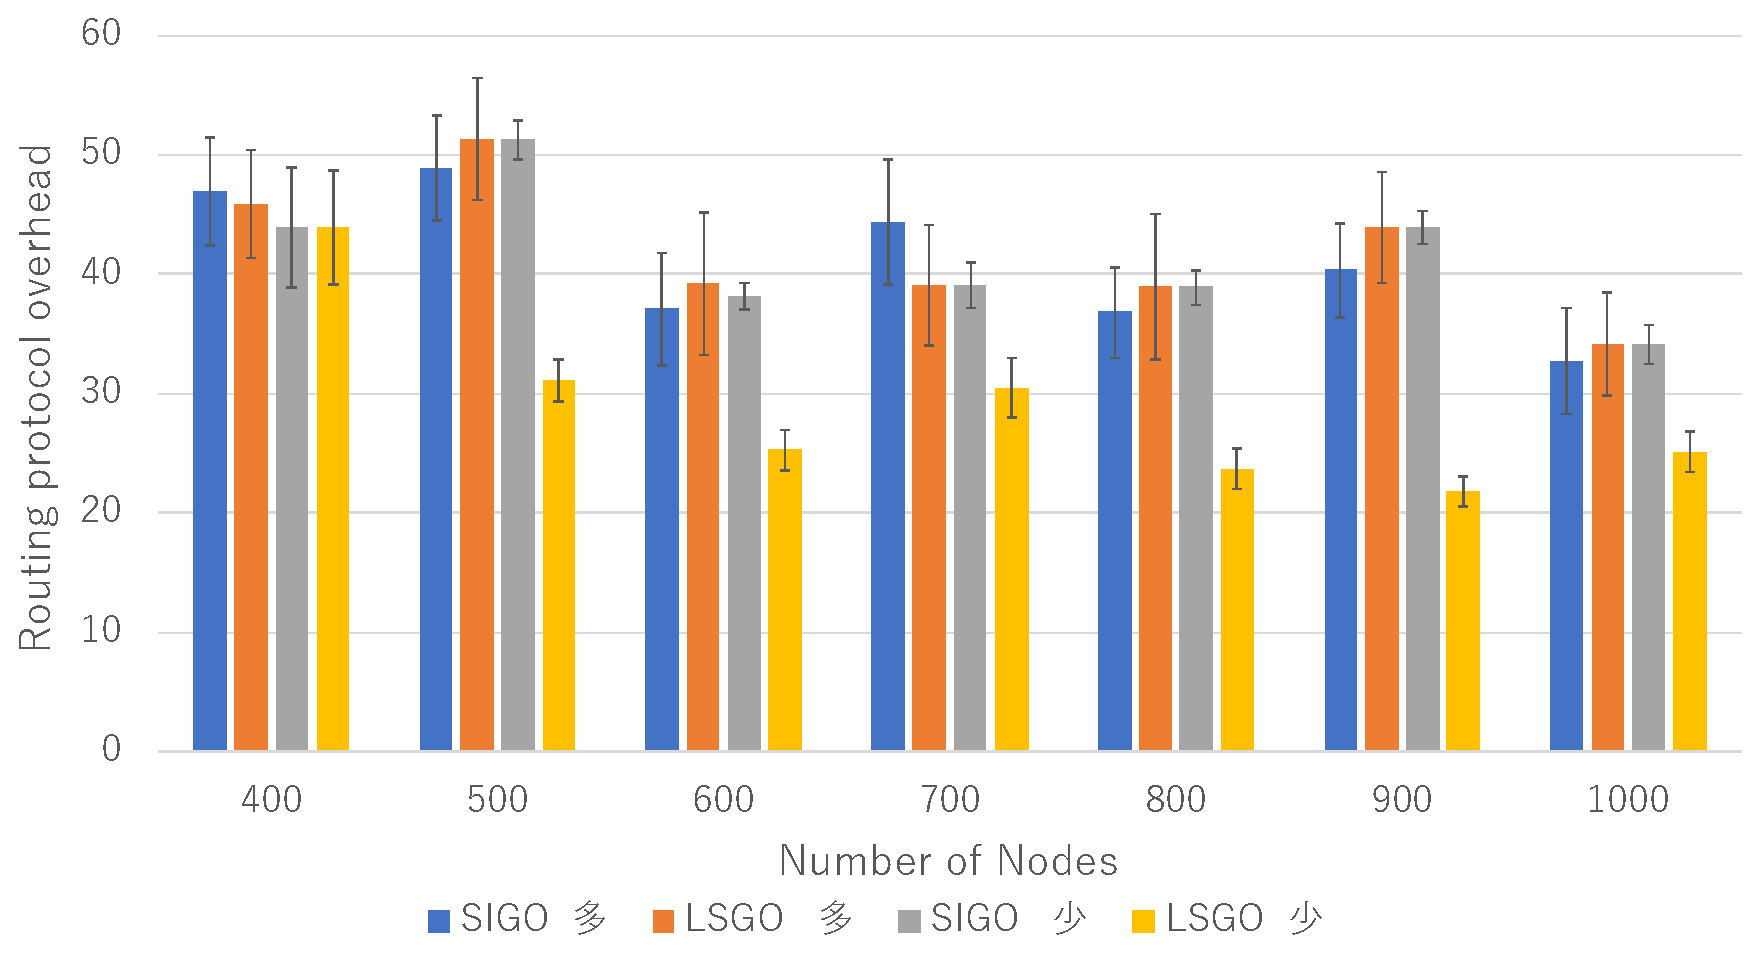
\includegraphics[width=90mm]{figures/Overhead.eps}
\caption{オーバーヘッド LSGO vs SIGO}
\label{fig:Overhead}
\end{figure}

 \begin{figure}[!ht]
\centering
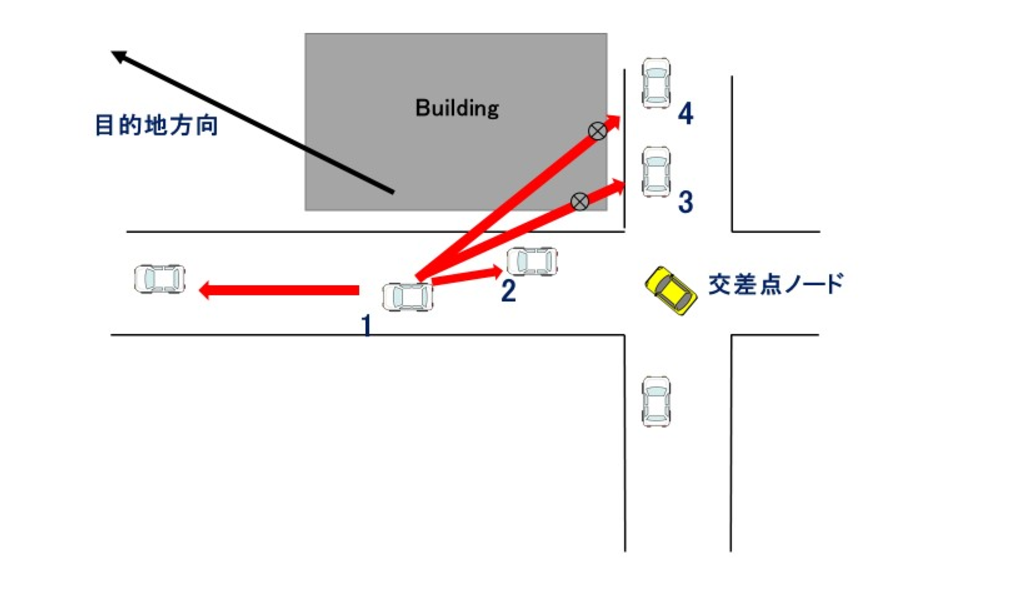
\includegraphics[width=90mm]{figures/Overhead-reason.eps}
\caption{オーバヘッド増加原因の例}
\label{fig:Overhead-reason}
\end{figure}





\section{まとめ}
本研究では, 既存opportunistic routingがシミュレーションでシャドウイングに対する影響を評価できていない問題, またそれによってルーチングプロトコルを設計するにあたってシャドウイングの影響を考慮できていないという問題に着目し,シミュレーションでシャドウイングを考慮した評価を行った. 既存ルーチングプロトコルはシミュレーションでシャドウイングに対する影響を評価した場合, 通信性能が低下することを示した. また, シャドウイングの影響を受けにくいルートを形成するSIGOを提案し, パケット到達率の向上, エンドツーエンド遅延の減少を確認し, 有効性を示した. しかし, 建物が少なくシャドウイングが起こりにくいシナリオでは既存 ルーチングプロトコルと比較して, エンドツーエンド遅延, オーバーヘッドが増加する可能性が高いという傾向がみられた. 今後は, ノードの優先度を求めるだけでなく道路の優先度を決定することで冗長なパケットを防ぐことや, Hello パケットの情報を利用し, シャドウイングの影響の大きさを推測し, 交差点度数の重みづけαを定数ではなく, 道路状況によって適応的に設定するなどの対策が必要だと考える. 




\begin{thebibliography}{99}
% \bibitem{A}IBM セキュアなIoTソリューションの設計と構築
% \url{https://www.ibm.com/developerworks/jp/iot/library/iot-trs-secure-iot-solutions2/index.html}
% \bibitem{B}吉田耕太, 西村浩二, 大東俊博, 相原玲二 : 秘密分散法を利用したクラウドストレージサービスにおけるモバイル機器を考慮した安全な処理委託方式 情報処理学会論文誌, Vol.55, No.3, pp.1117-1125(Mar. 2014)
% \bibitem{C}Javier Munster, Hans-Arno Jacobsen : Secret Sharing in Pub/Sub Using Trusted Execution Enviroments, DEBS'18, June 25-29, 2018
% \bibitem{D}松尾正克, 古賀田勝則, 田中裕之, 武藤浩二, 小林正明 : IoT機器のための暗号・認証技術, およびサイバー攻撃検知, 対策技術, Panasonic Technical Journal, Vol.64, No.1, May 2018
% \bibitem{E}木村一統, 新井イスマイル, 藤川和利 : MQTT-SNの実装評価, 「

\bibitem{ITS}	国土交通省道路局:ITS スポット(オンライン),入手先
\url{http://www.mlit.go.jp/road/ITS/j-html/spot dsrc/ index.html}

% 著者名,"標題," 会議名,no.を付けて論文番号,pp.を付けて始め-終りのページ,開催都市名,国名,月年.

\bibitem{Old1}Lochert, C., Mauve, M., Fussler, H. and Hartenstein, H."Geographic Routing in City Scenarios", ACM SIGMO- BILE Mobile Computing and Communications Review, Vol.9, No.1, pp.69–72 ,2005.
\bibitem{Old2}	H. Tong, Nonlinear Time Series" A Dynamical System Approach", J. B. Elsner, ed., Oxford University Press, Oxford, 1990.
\bibitem{EXOR}	S Biswas, R Morris, "ExOR: opportunistic multi-hop routing for wireless networks", in Proceedings of the 2005 Conference on Applications, Technologies, Architectures, and Protocols for Computer Communications, Philadelphia, pp. 133–144, August 2005. 
\bibitem{LSGO} 	Uelian Cai, Ying He, Chunchun Zhao, Lina Zhu, and Changle Li, "Lsgo: Link state aware geographic opportunistic routing protocolfor vanets", EURASIP Journal on Wireless Communications andNetworking, Vol. 2014, No. 1, p. 96, June 2014.
\bibitem{Obstacle} 	S. E. Carpenter and M. L. Sichitiu, “An obstacle model implementa- tion for evaluating radio shadowing with ns-3,” in Proc. WNS, pp.17–24, May 2015.
\bibitem{GPSR} 	B Karp, HT Kung, "GPSR: greedy perimeter stateless routing for wireless networks", in Proceedings of Mobile Computing and Net-working, Boston, pp. 243–254, August 2000
\bibitem{GPCR}	C Lochert, M Mauve, H Füssler, H Hartenstein, "Geographic routing in city scenarios", in Proceedings of the SIGMOBILE Mobile Computing and Communications Review, vol. 9(1), pp. 69–72, 2005.
\bibitem{ETX} DSJ De Couto, D Aguayo, J Bicket, R Morris, "A high throughput path metric for multi-hop wireless routing", in Proceedings of the 9th Annual International Conference on Mobile Computing and Networking (MobiCom’ 03), San Diego, pp. 134–146, September 2003.
\bibitem{SCAOR}Sadatpour, V, Zargari, F Ghanbari, M , "A Collision Aware Opportunistic Routing Protocol for VANETs in Highways",  Wireless Personal Communications 109, 175–188, springer 2019.
\bibitem{NS3} Network Simulator ns3, https://www.nsnam.org
\bibitem{SUMO} Simulation of Urban Mobility, https://sumo.dlr.de/docs/index.html 
\end{thebibliography}



\end{document}
